\section{Results}\label{sec:results}
\begin{table}[!t]
\caption{Classifiers with top 5 testing accuracy combined with baseline and augmentation results.}
\label{tab:table2}
\scalebox{0.68}{
\begin{tabular}{ccccccc}
\toprule
\multicolumn{1}{l}{} Rank & Classifiers   & Data Type & Transformation & Augmentation & GAN & \multicolumn{1}{l}{Accuracy} \\ \hline
1                    & XGB           & Raw       & Yes            & SMOTE        & No  & 0.739                        \\
2                    & Random Forest & Raw       & Yes            & SMOTETomek   & No  & 0.730                        \\
3                    & MLP           & Raw       & No             & TomekLinks   & Yes & 0.727                        \\
4                    & XGB           & Raw       & Yes            & SMOTETomek   & No  & 0.726                        \\
5                    & Decision Tree & Raw       & No             & SMOTE        & No  & 0.725                        \\ \bottomrule
\end{tabular}
}
\end{table}

\begin{figure*}[t!]
    \centering
    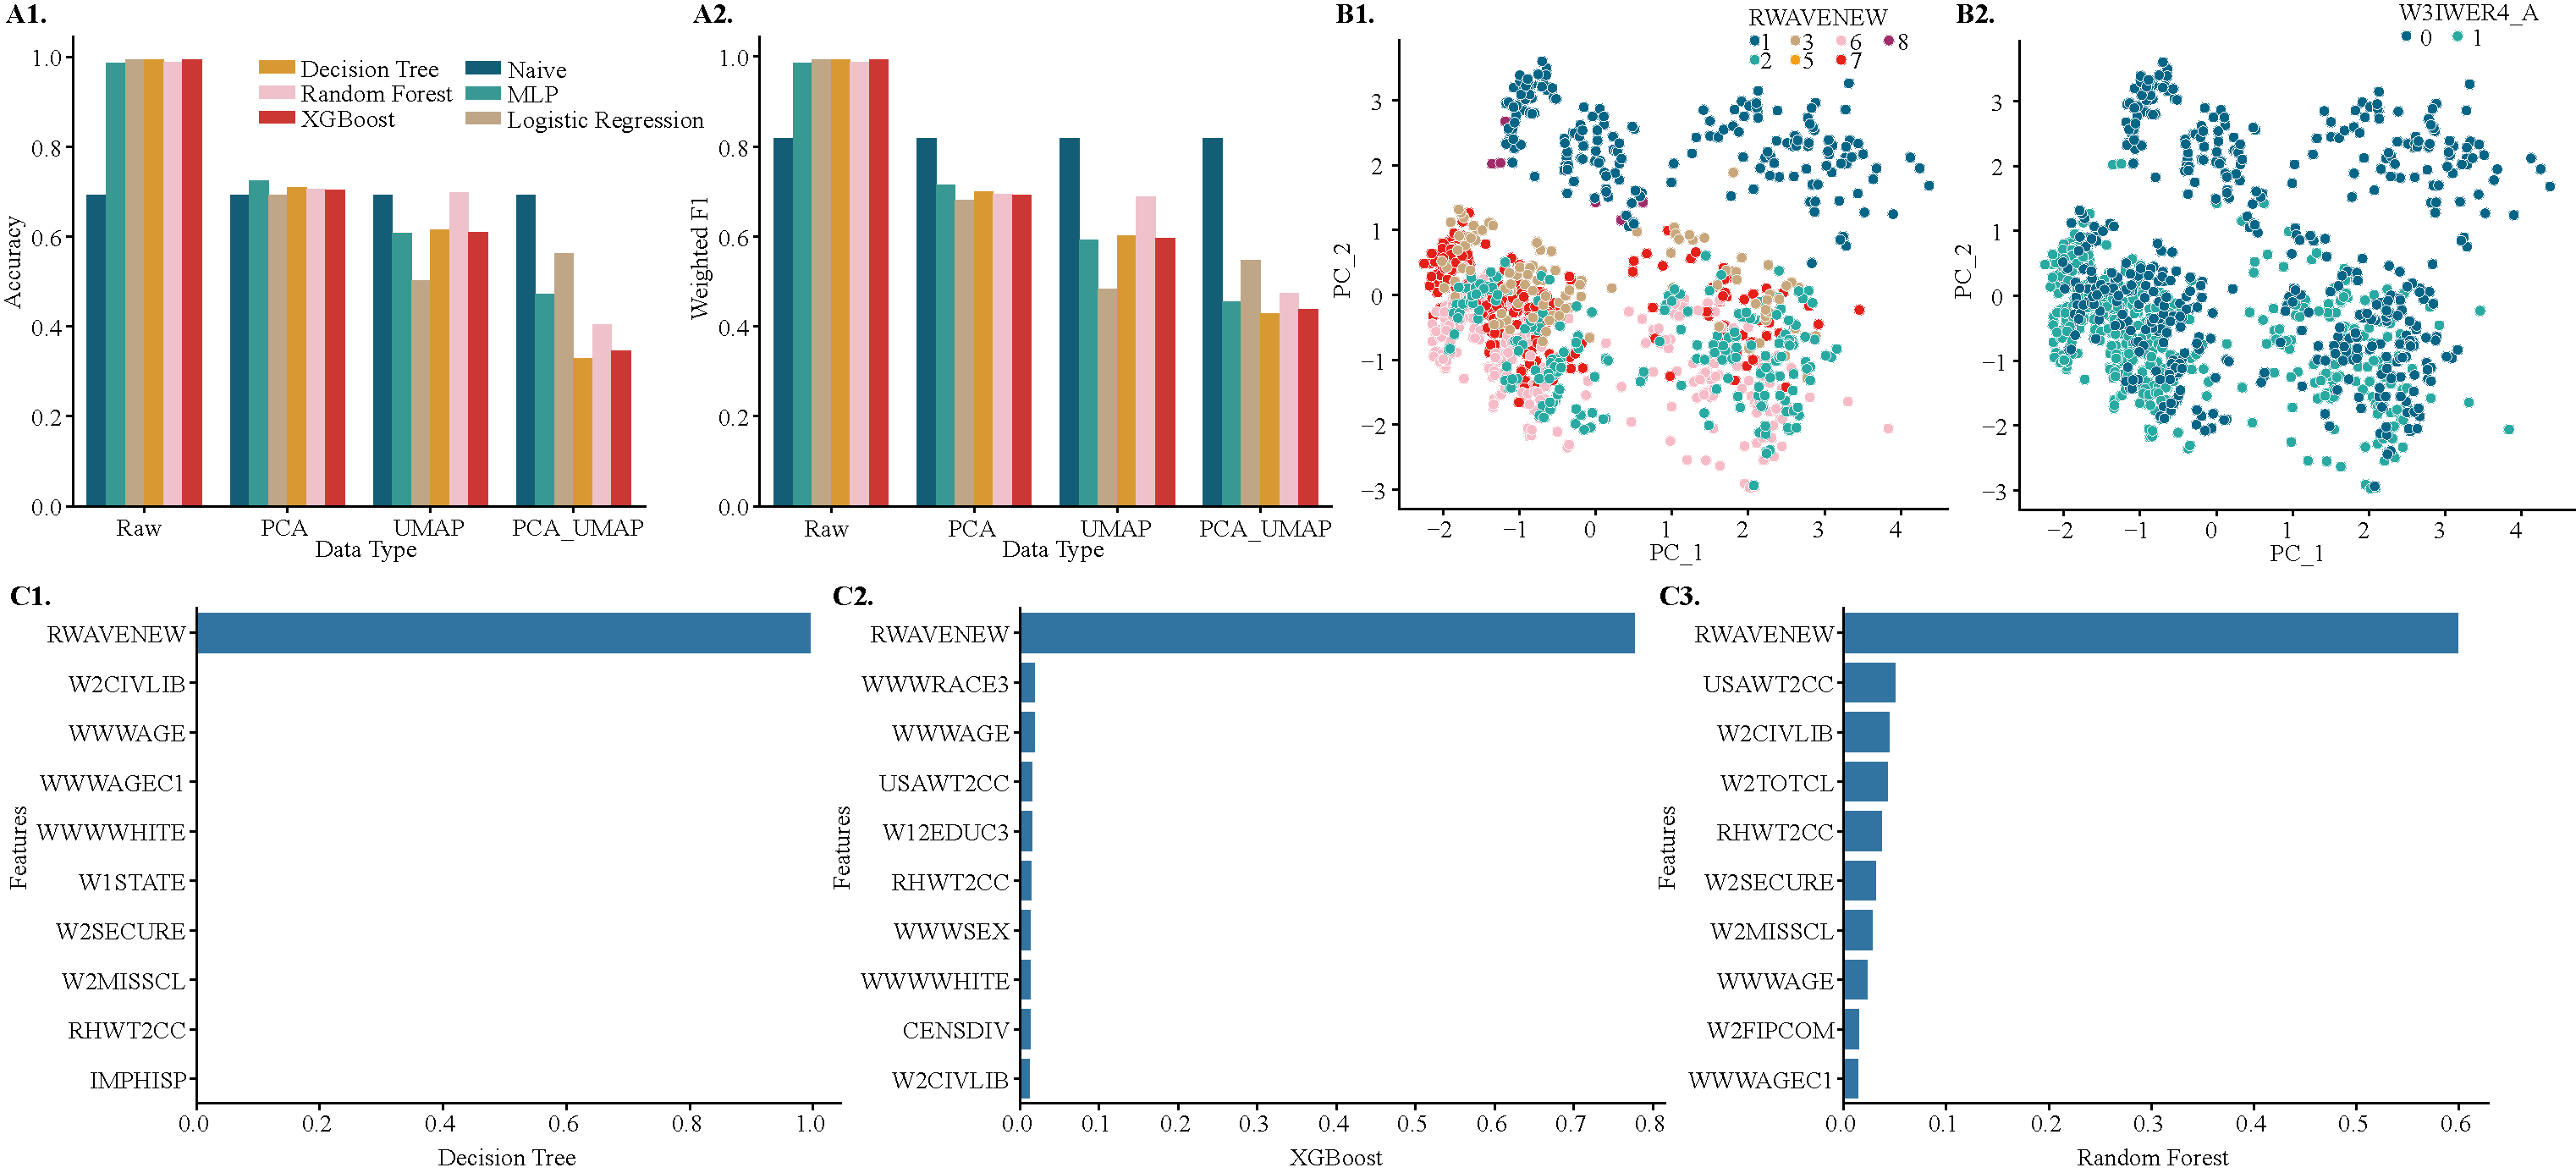
\includegraphics[width=\linewidth]{Figures/Figure2.pdf}
    \caption{Experimental results for batch effects exploration. Shown are the bar plots of test (A.1) accuracy and (A.2) weighted F1 score of the prediction of six classifiers with four data types, scatter plots of two dimensional principal components of the training dataset labelled by the (B1.) batch and (B2.) label, and horizontal bar plots of the training feature importance obtained by the (C1.) Decision Tree, (C2.) XGBoost, and (C3.) Random Forest. Top 10 features are retained. }
    \label{fig:figure2}
\end{figure*} 

\begin{figure*}[t!]
    \centering
    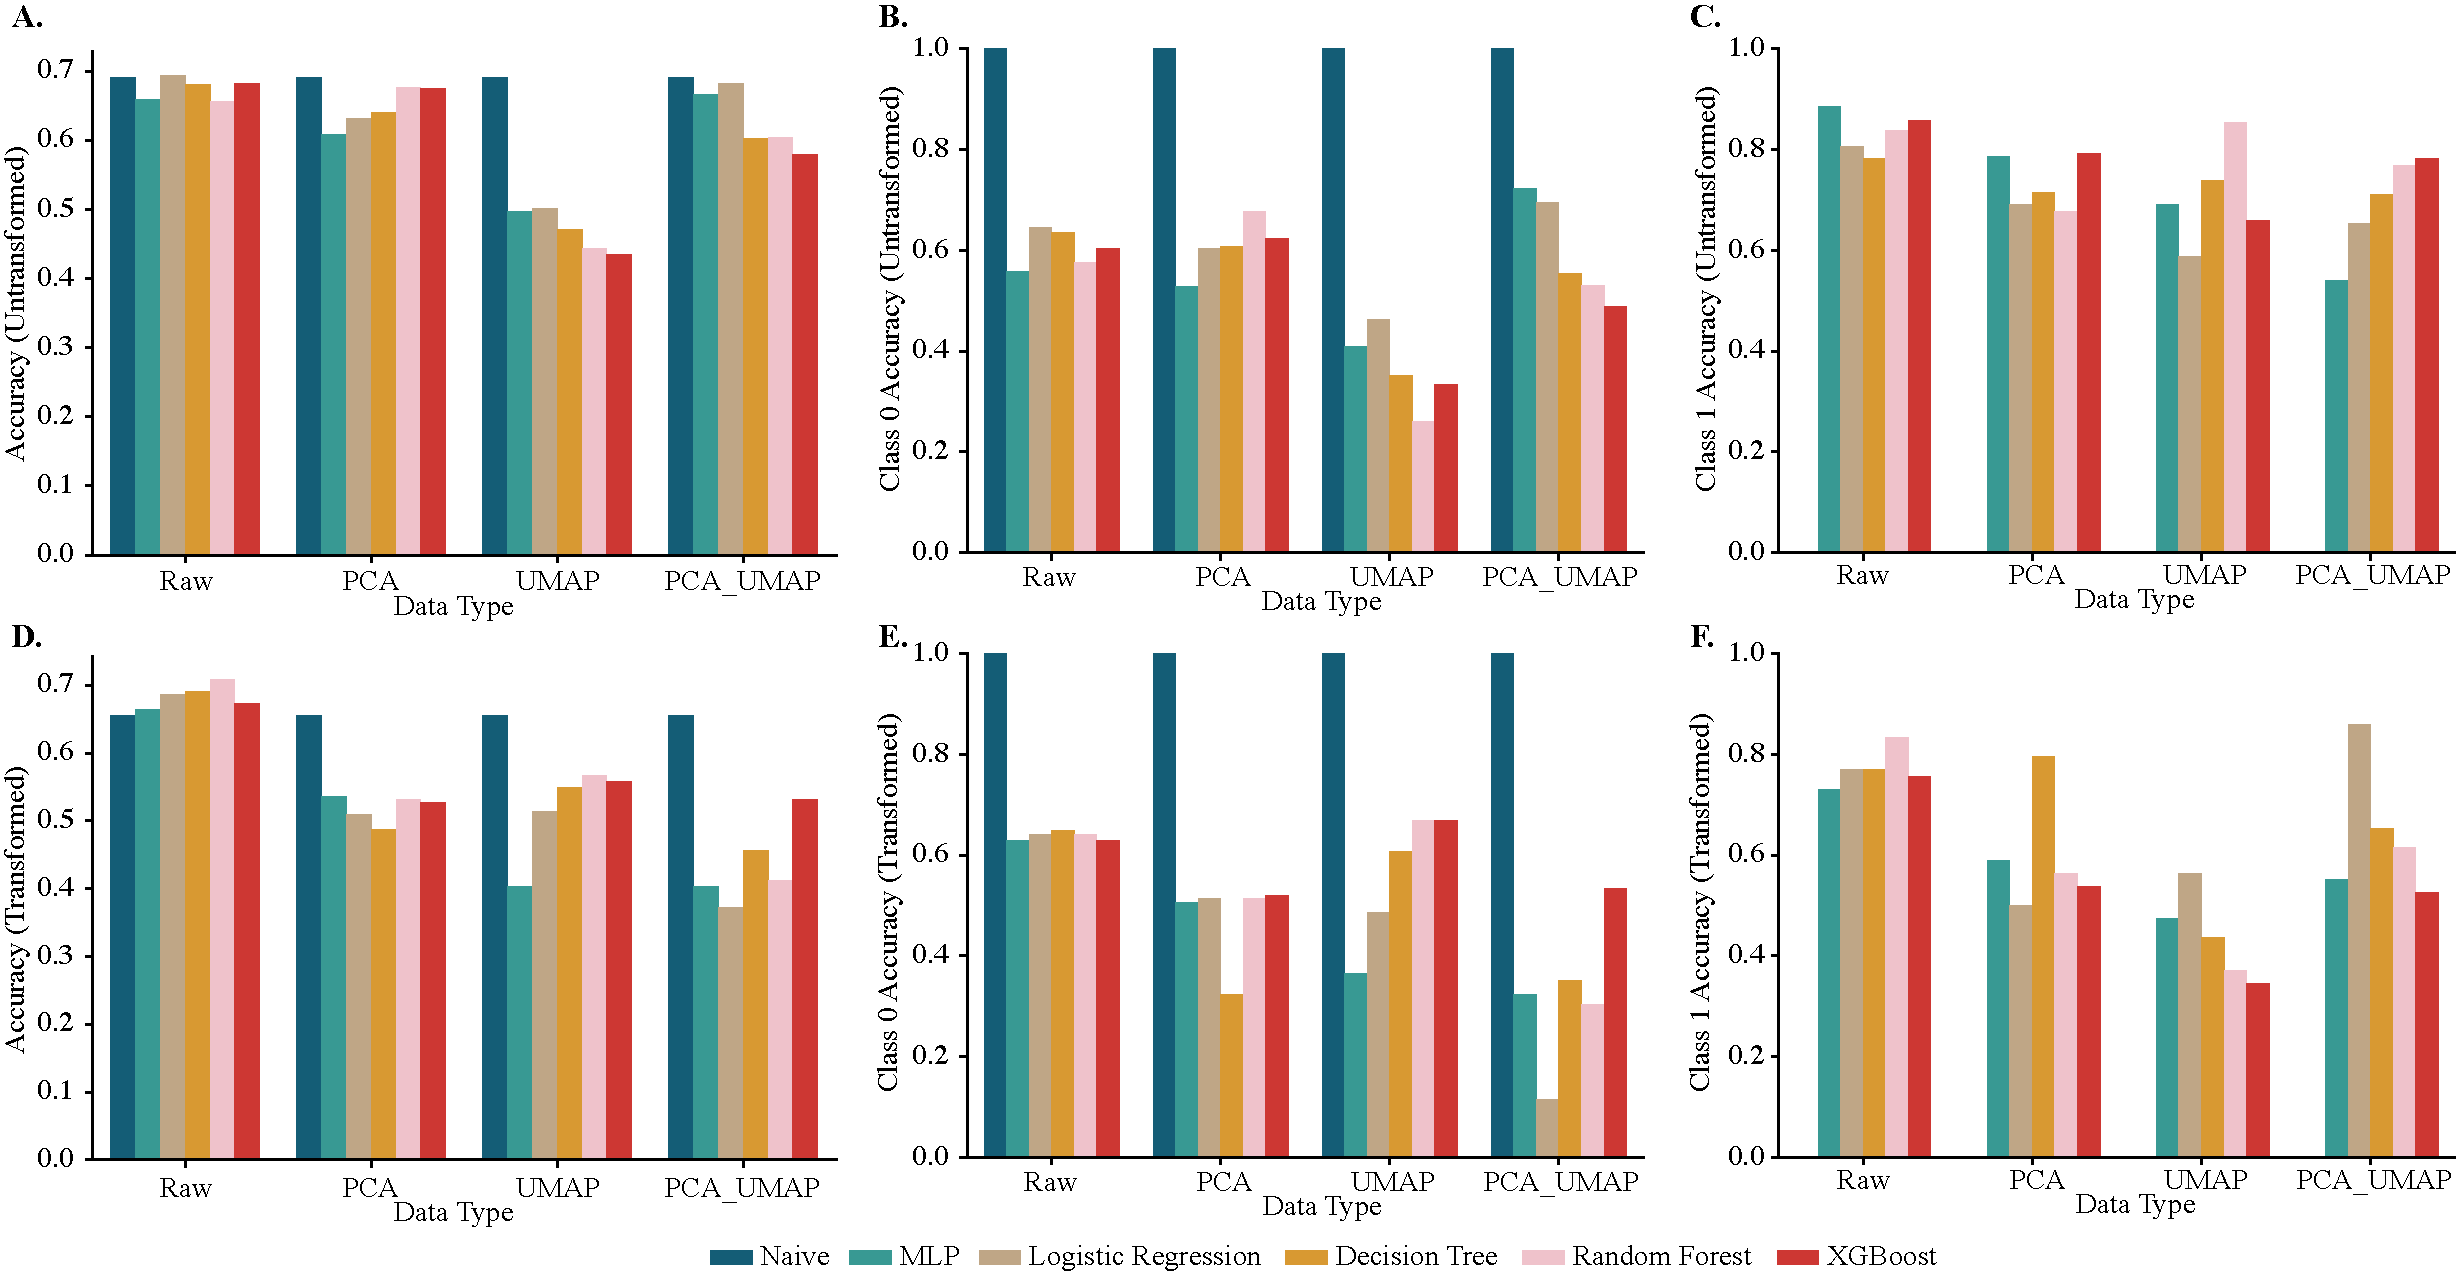
\includegraphics[width=14cm]{Figures/Figure3.pdf}
    \caption{Baseline experimental results. Shown are the bar plots of (A, D) test accuracy, (B, E) class 0 accuracy, (C, F) class 1 accuracy of the (top) untransformed and (bottom) transformed data. Each plot contains classification performance of six classifiers including naive approach with four data types.}
    \label{fig:figure3}
\end{figure*} 

\begin{figure*}[t!]
    \centering
    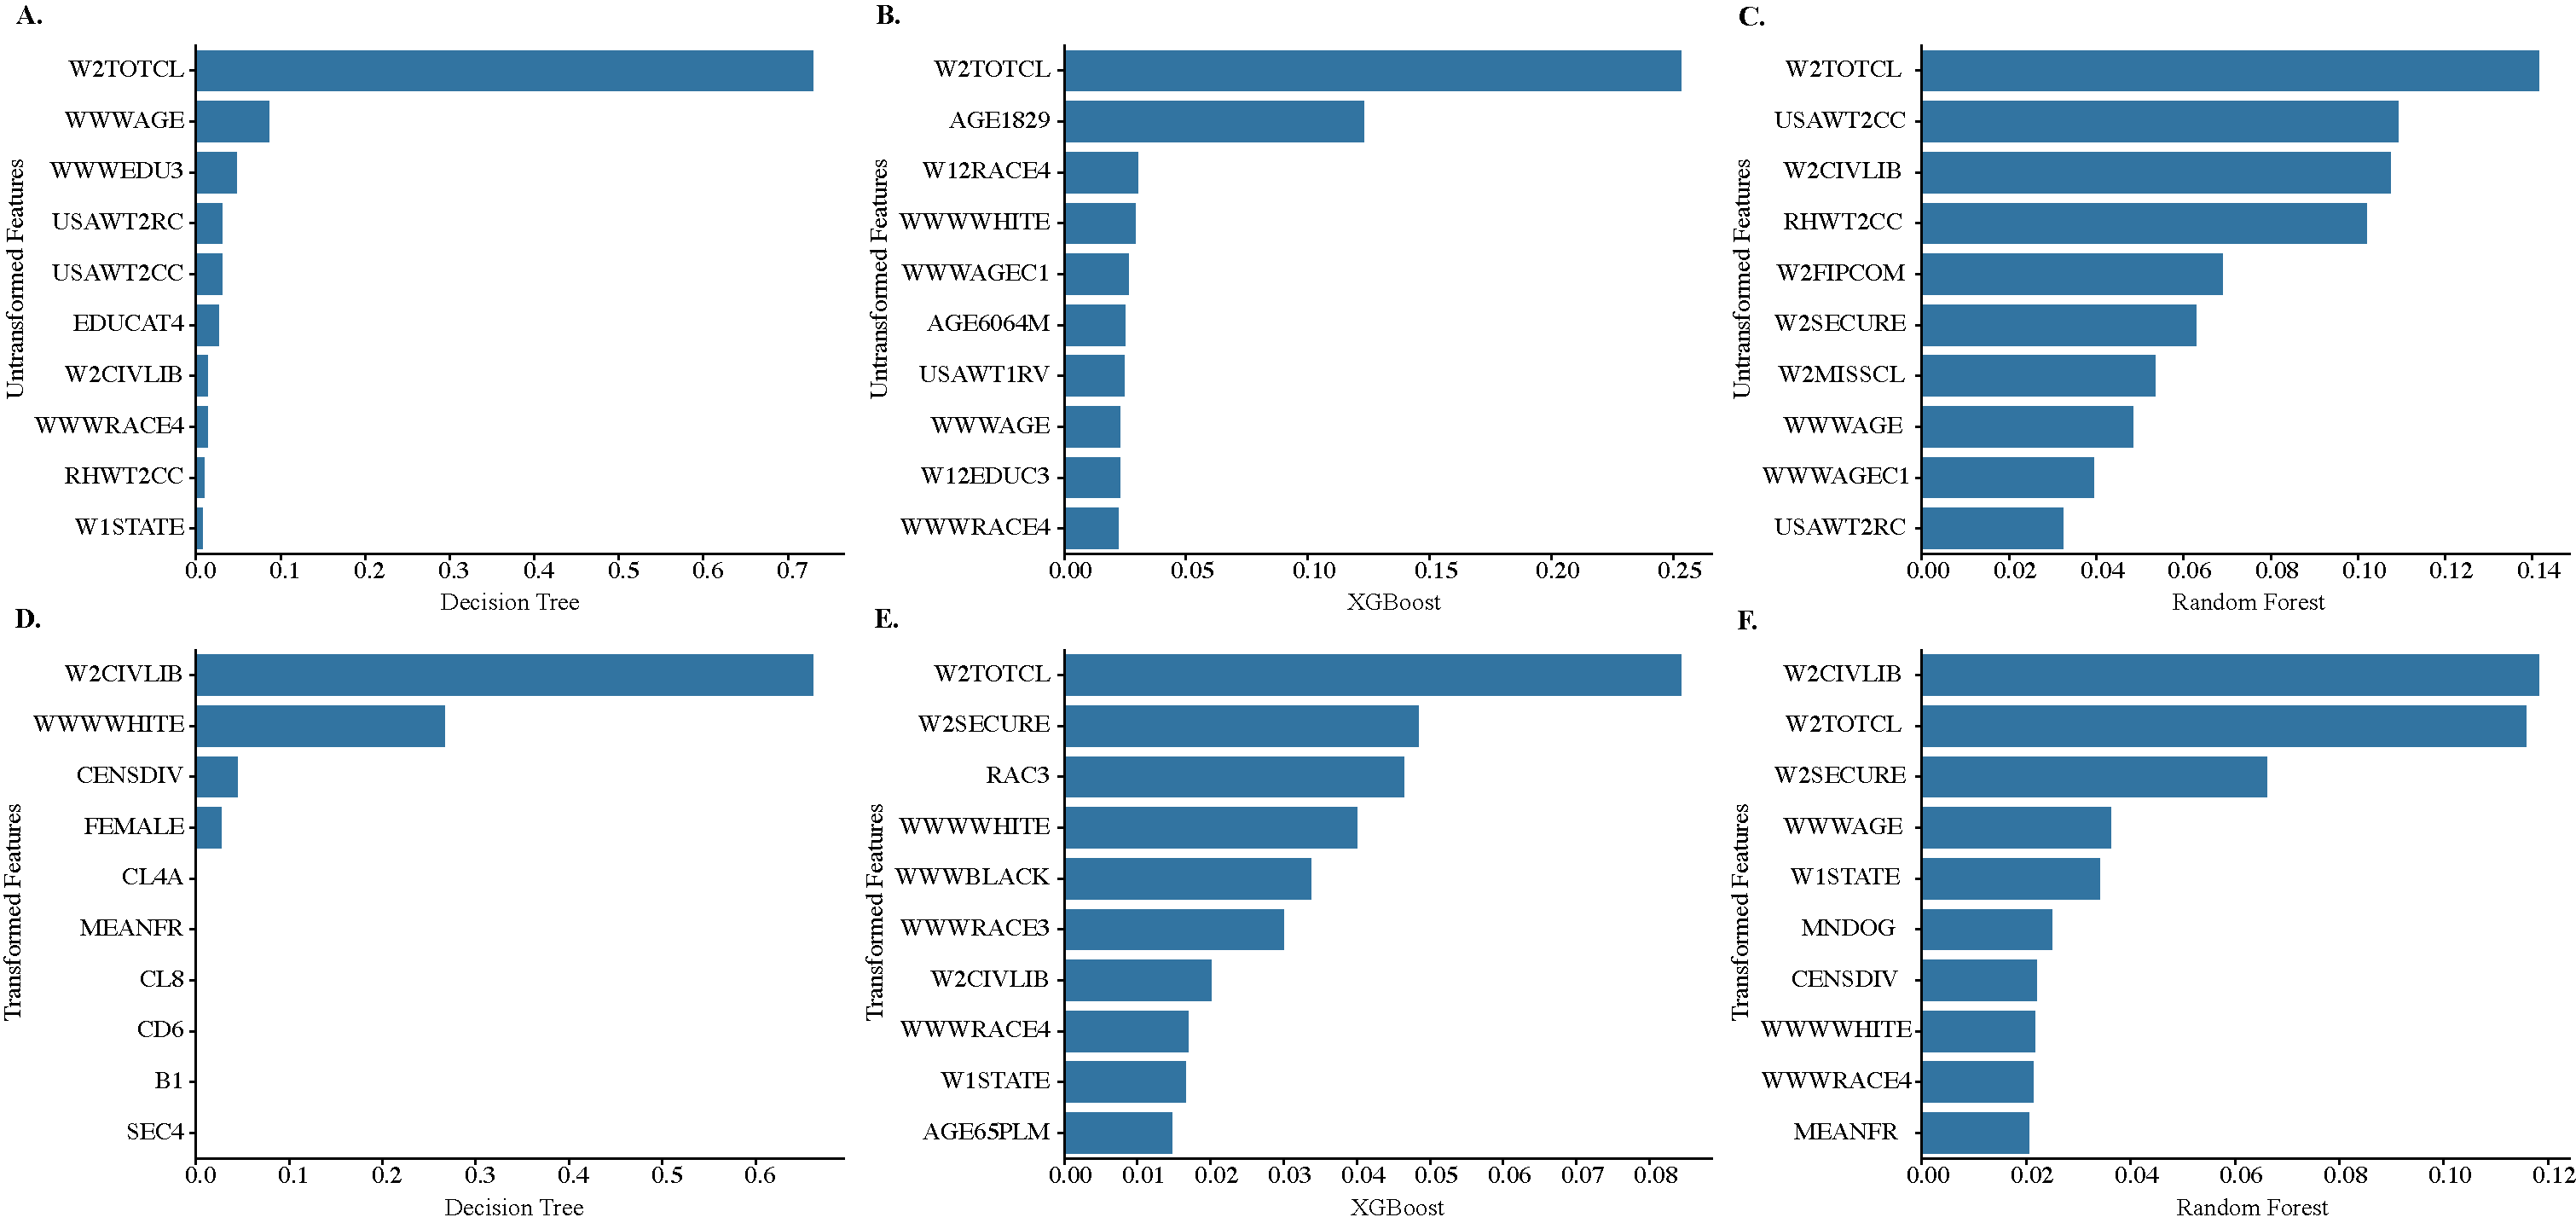
\includegraphics[width=14cm]{Figures/Figure4.pdf}
    \caption{Feature importance for baseline experiments. Shown are the horizontal bar plots of the feature importance of (top) untransformed and (bottom) transformed data predicted by (left) Decision tree, (middle) XGBoost, (right) Random Forest.}
    \label{fig:figure4}
\end{figure*} 

\begin{figure*}[t!]
    \centering
    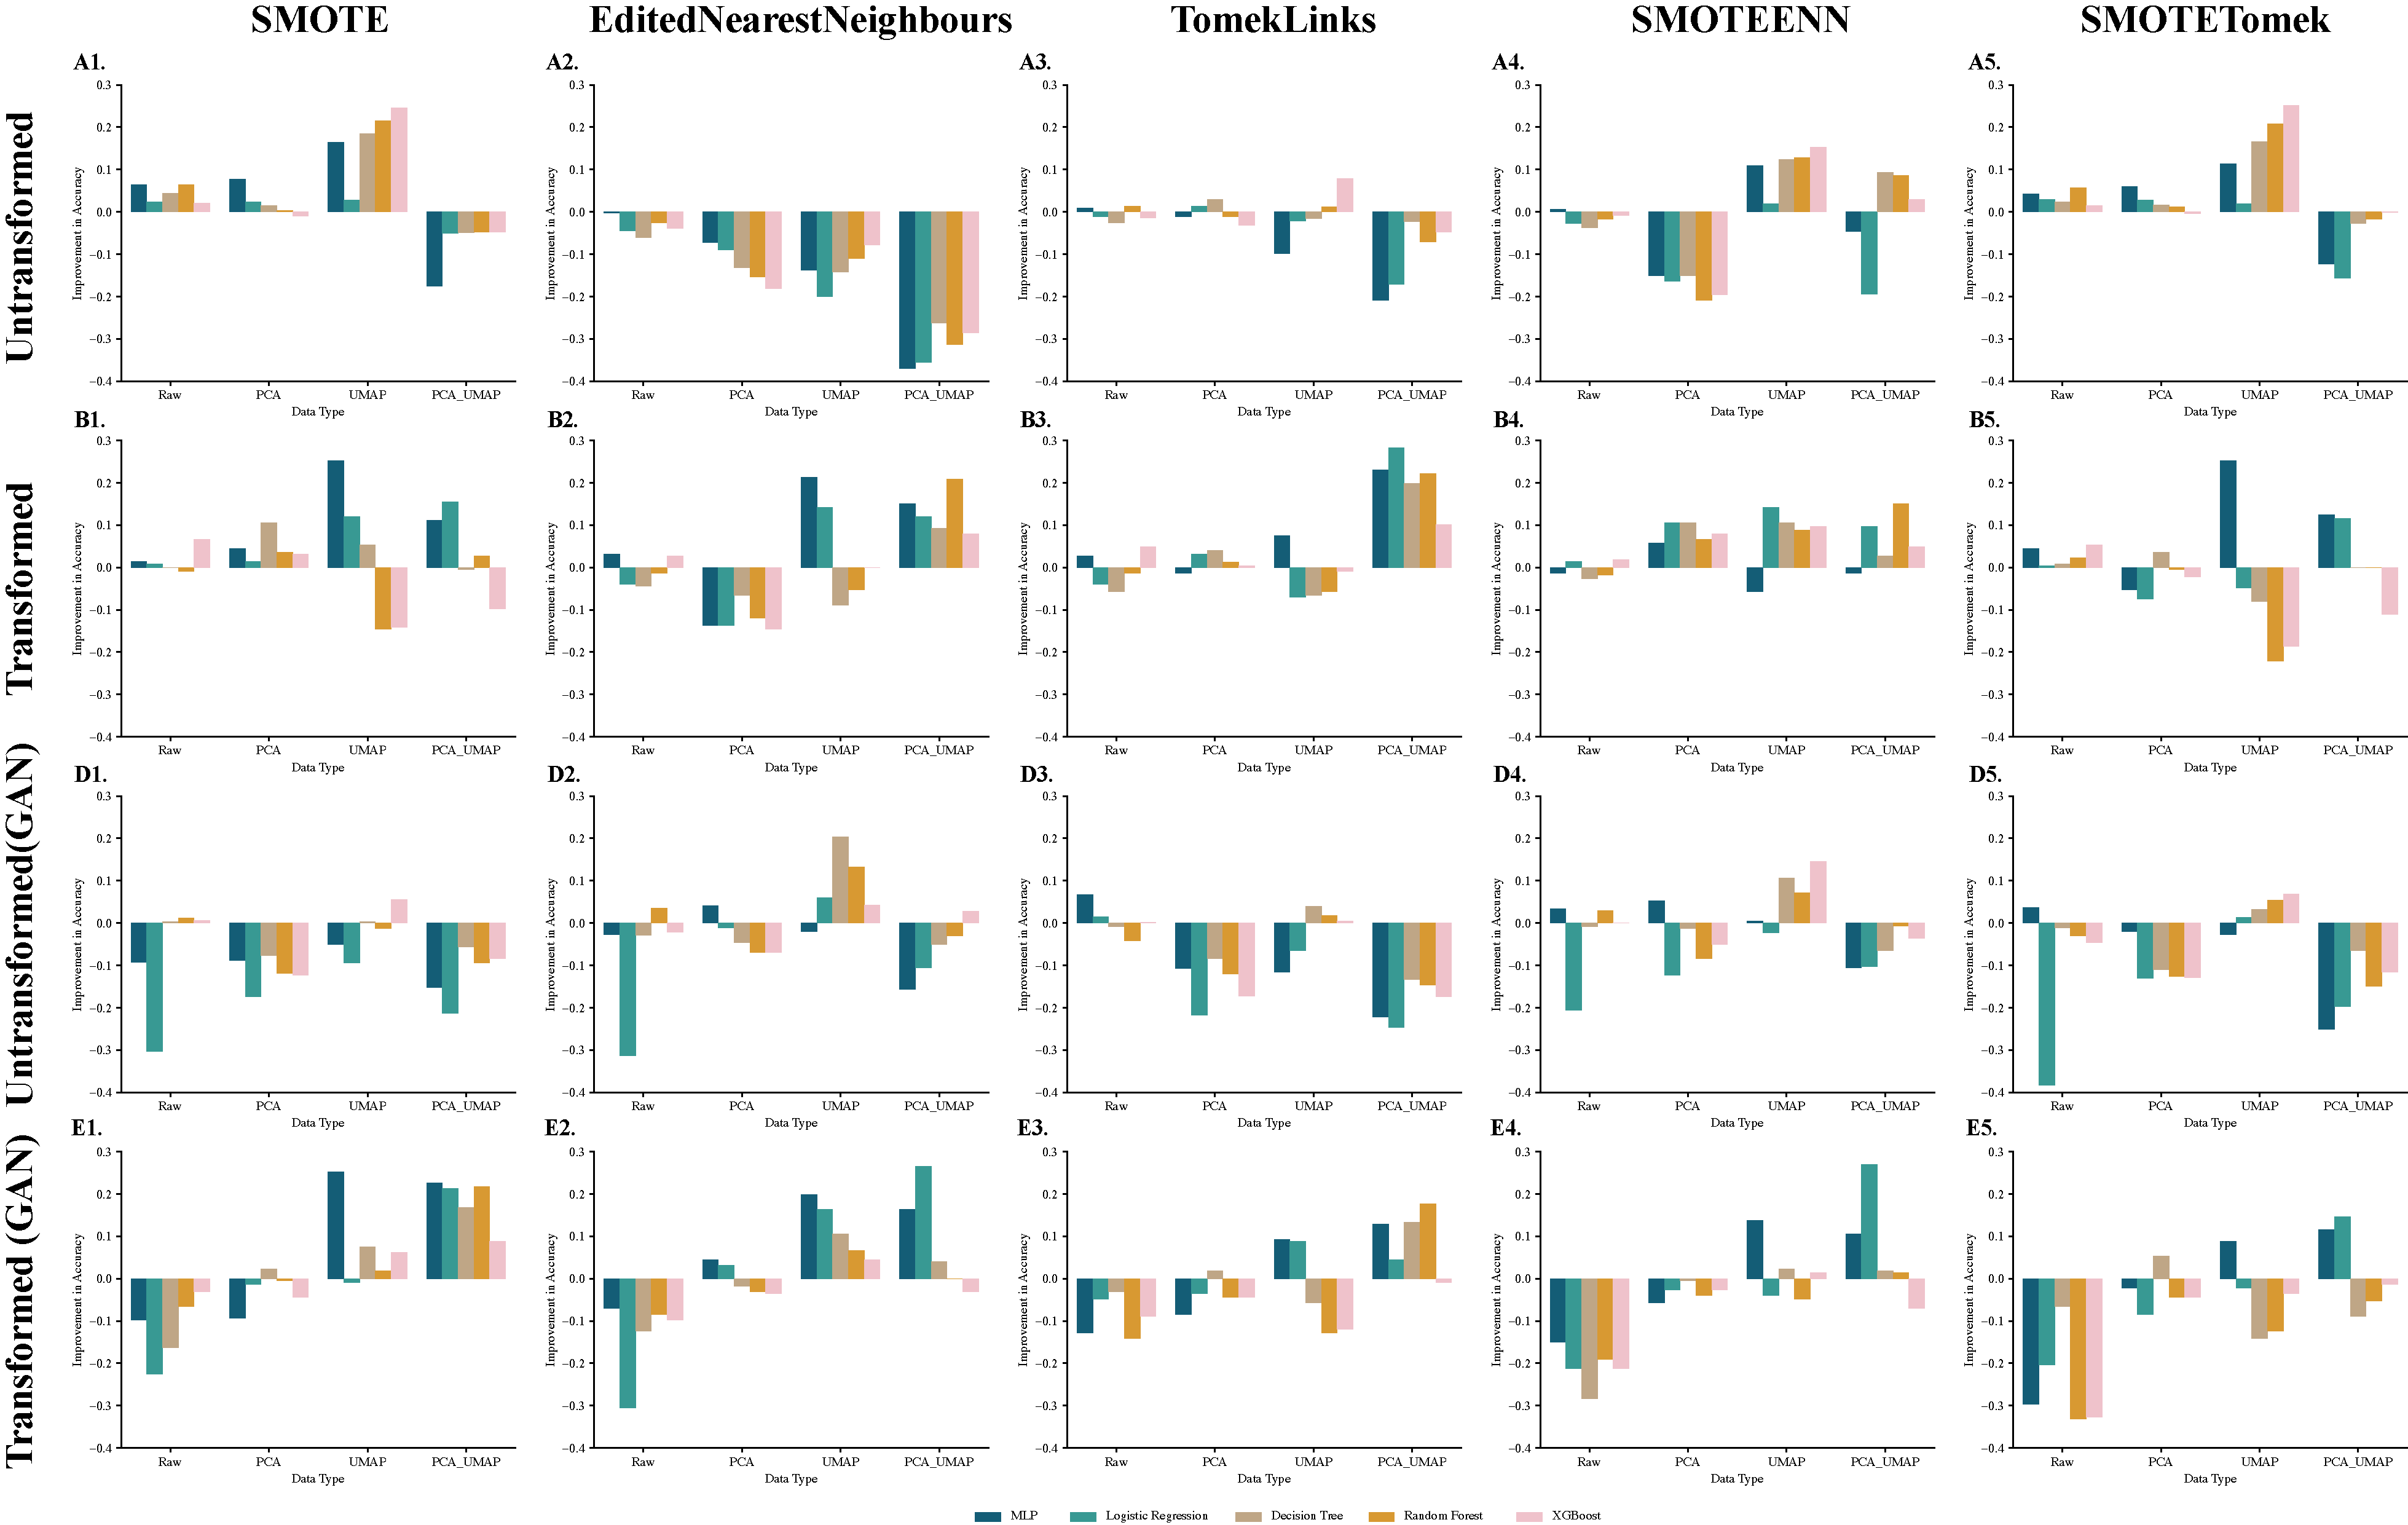
\includegraphics[width=\linewidth]{Figures/Figure5.pdf}
    \caption{Results for benchmarking data augmentation methods. Shown are the bar plots of the improvement in accuracy after applying data augmentation methods compared to the baseline results. Five sampling data augmentation methods are tested with (A.) untransformed data and (B.) transformed data. (C.) and (D.) demonstrated the improvement in performance after augmenting GAN to each of the sampling-based data augmentation method with untransformed and transformed data, respectively.}
    \label{fig:figure5}
\end{figure*}

The results demonstrate the flexibility and easy use of the framework to explore meaningful patterns, provide baseline results, and benchmark data augmentation methods. We found two variables which caused batch effects in our dataset. Using our proposed data transformation method, we show that our method is well suited to resolve batch effect without sacrificing performance. Our method also provides more meaningful interpretations, where we have empirically shown that data augmentation methods can improve the performance of classifiers for some datasets. For each of the experiment, we include datasets with four data types (Raw, PCA, UMAP, and PCA\_UMAP).

\textbf{A batch effect by wave-related variable is discovered.} When classifying the cooperativeness of the respondents from the original data features. We found that the performance of each classifiers is unreasonably high with raw data, where the average accuracy is 0.993$\pm$0.405 and the weighted F1 is 0.991$\pm$0.404 (figure ~\ref{fig:figure2}A). With such a phenomena, we suspected that batch effects might exist that affect the decision boundary of the classifiers. We therefore, computed the training feature importance of each feature by Decision Tree, XGBoost, and Random Forest (figure ~\ref{fig:figure2}C). We found a dominating variable RWAVENEW whose feature importance is significantly higher than the rest of the features. The variable RWAVENEW indicates the wave of the survey the respondents have participated in, and it seems that an inherent cluster exist by the RWAVENEW variable that guides the learning of classifiers. We confirmed our findings by creating the scatter plot of the training data labelling by the suspected variable and the training label (figure ~\ref{fig:figure2}B). The results demonstrate that an cluster exist in the training that is not only based on the label but also on the batch RWAVENEW. Interestingly, after dimensionality reduction, the effect of batch effects is slightly mitigated as a significant drop in performance could be observed in any of PCA, UMAP, or PCA\_UMAP data. We hypothesize that this behavior might be due to dimensionality reduction techniques that reduce the noises of the batch variable and make them less standing out in lower dimensions.

Since the purpose of this study is to find the cooperativeness of the respondents solely from their answers, we classify this phenomenon as a batch effect by the wave-related variable. We further examined our dataset and found a variable RWAVEOLD that is highly correlated to RWAVENEW, and it generated similar results to RWAVENEW. Therefore, to remove batch effects we remove RWAVENEW and RWAVEOLD in rest of our experiments, where the dataset is called untransformed dataset. In addition, since the dataset contains responses from three waves, we also proposed a data transformation method that further mitigates the batch effect by only obtaining the variables of the first wave that the respondents are interview in, which reduces the dimensionality, where the dataset is called transformed data. 

In rest of the experiments, we tested on different combination of both untransformed and transformed data with different data types. In addition, since weighted F1 generates similar patterns to accuracy and we still want to consider each class equally though a class imbalance exists in the testing data, we only use accuracy and class accuracy to evaluate the performance of classifiers.

\textbf{The proposed data transformation method could provide a more meaningful explanation to the features contributing to the prediction of cooperativeness while not sacrificing the performance.} The results demonstrating that the average classification accuracy across 5 classifiers not including naive classifier is not significantly different, where the averaged accuracy of prediction is 0.674 $\pm$ 0.163 on untransformed data and is 0.684 $\pm$ 0.0917 for transformed data (figure \ref{fig:figure3} AD). Although the class imbalance of testing data is different from transformed and untransformed data, the performance of 5 classifiers outperforms the naive classifier and demonstrates the superiority of transformed dataset in its own context. However, the performance of classifiers in transformed dataset drops significantly compared to the untransformed dataset except for UMAP, where the average accuracy (0.518 $\pm$ 0.067) of transformed data in UMAP significantly outperforms the average accuracy (0.469 $\pm$ 0.030) of untransformed data in UMAP, demonstrating that a non-linear reduction technique might be better at capturing the internal data structure in the transformed data. Whereas, in untransformed data, interestingly, PCA reduction and PCA\_UMAP reduction does not significantly decrease the performance of classifiers except for UMAP reduction, indicating that a linear relationship exist in the dataset that if one wants to use a dimensionality reduction technique to reduce the features, a linear relationship must be captured.

In addition,, the classification accuracy of class 1 (figure \ref{fig:figure3} BE) which is the label cooperative is significantly higher than the classification accuracy of class 0 (figure \ref{fig:figure3} CF) which is the label uncooperative. The label cooperative is the minority class in the testing dataset and we hypothesize that in the testing data, a cluster might exist based on the label of cooperative which makes classifier easier to distinguish compared to uncooperative. A more detailed technical attribution is presented in discussion section. Additionally, the results show that tree-based classifiers are better at classifying the uncooperative except for a significantly high performance by logistic regression in transformed data with PCA\_UMAP reduction.

The transformed dataset produces more meaningful explanations of the feature importances since the models were not dominated by one feature. In the models trained on untransformed data in figure ~\ref{fig:figure4} ABC, W2TOTCL is far and above the most important feature in each model. In decision trees and XGBoost, W2TOTCL severely impacts the classification of a sample. In the models trained on transformed data in figure ~\ref{fig:figure4} DEF, the drop off in feature importance after the most influential features is much less. Although the decision tree is still dominated by one attribute, in XGBoost a significant scale shift is observed. For the XGBoost model trained on transformed data the most important feature importance was about 0.08; whereas, for the XGBoost model trained on the untransformed data the most important feature was about 0.25.

It is worth noting that the feature which models A, B, and C identify as the most influential feature for whether a respondent takes the survey seriously appears to be an example of overfitting. Models A, B, and C all identify W2TOTCL as the most important feature; however, this feature tracks how many questions a respondent favored civil-liberties in. Since the models appear to be overfitting on W2TOTCL, they are under-valuing the importance of other features yielding a less meaningful interpretation of feature importances. In the Discussion section, we will further explain why we believe our models trained on untransformed data to be overfitting.

\textbf{Data augmentation methods improve performance with low-dimensional training data, and the best classifier for classifying the cooperativeness of survey respondent is created by augmented and transformed training data.} In general, data augmentation methods are more effective in UMAP (0.03$\pm$0.118) and PCA\_UMAP (-0.0119$\pm$ 0.148) data compared to Raw (-0.05$\pm$0.103) and PCA (-0.04$\pm$0.075) data by improvement in accuracy across all data and methods (figure ~\ref{fig:figure5}). Despite the negative overall improvement in PCA\_UMAP data, its large standard deviation suggests that the augmentation methods are indeed effective in most of the dataset for PCA\_UMAP data. Considering UMAP and PCA\_UMAP data, SMOTE (0.035$\pm$0.130) and SMOTENN (0.040$\pm$0.090) are the best data augmentation methods having top two improvements in accuracy. However, GAN is not effective when augmenting to each of the sampling-based data augmentation methods except for editENN with a average improvement in accuracy of 0.056$\pm$0.107 across both transformed and untransformed data. We attributed this behavior to the over down-sampling by the editENN as it can be observed from figure ~\ref{fig:figure5} A2. where editENN significantly drops the performance. Therefore, by increasing the size of the training data, GAN is more effective when augmented with the editENN. Although across transformed and untransformed data, GAN is not effective in improving the performance, it performs differently in transformed data than untransformed data. In transformed data, GAN improves the average accuracy by 0.060$\pm$0.108 compared to the -0.045$\pm$0.102 of untransformed data. The reason is that after transformation, the size of the training data is significantly smaller than the size of training data with untransformed data as shown in table ~\ref{tab:table1}.

After data augmentation, combining baseline performance, the best classifier is XGB with raw, transformed, and augmented data, having a accuracy of 0.739 (table ~\ref{tab:table2}). Interestingly, the top two classifiers both take transformed data as input, and both of the classifiers use augmented training data. Therefore, we conclude that the performance of classifiers in classifying cooperativeness in survey is improved by applying data transformation and augmentation techniques. 




